\section*{\nr.3 \titthree (25 Punkte)}
\begin{enumerate}[(a)]
\item Die Superposition der gegebenen Wellenfunktionen sich durch
\begin{equation}
\psi(x) = \cos{\alpha}\cdot\psi_{n,0}\cos{\left(\frac{\pi n x}{\lambda}\right)} + \sin{\alpha}\cdot\psi_{m,0}\cos{\left(\frac{\pi m x}{\lambda}\right)}
\end{equation}
gegeben. Zuerst wird die Normierung der Teilfunktionen ermittelt:
\begin{equation}
1 \overset{!}{=} \Braket{\psi_n (x)|\psi_n(x)} = \psi_{n,0}^2 \int_{-\lambda}^{\lambda}\mathrm{d}x \cdot {\cos^2{\left(\frac{\pi n x}{\lambda}\right)}} = \psi_{n,0}^2  \lambda
\end{equation}
Die letzte Gleichheit folgt unmittelbar aus der Symmetrie der $\cos^2$-Funktion. Es folgt (mit analoger Rechnung für das $m$-Funktionensystem) $\psi_{m,0} = \psi_{n,0} = 1/\sqrt{\lambda}$.

\item Nun wird die Normierung für die superponierte Wellenfunktion überprüft, wobei ausgenutzt wird, dass die oben definierten und normierten Funktionen $(\psi_j)_{j\in\mathbb{N}}$ ein orthonormale Hilbertraumbasis bilden:
\begin{align}
\Braket{\psi,\psi} &= \cos^2{\alpha} \Braket{\psi_n|\psi_n} + \sin^2{\alpha} \Braket{\psi_m|\psi_m} + 2 \sin{\alpha}\cos{\alpha}\Braket{\psi_n|\psi_m} \\
&= \cos^2\alpha + \sin^2 \alpha + 2\sin\alpha\cos\alpha \, \delta_{mn} = 1 + \delta_{mn}\sin {2\alpha}
\end{align}
Daran sieht man, dass die superponierte Wellenfunktion $\psi(x)$ nur für $n\neq m$ für alle $\alpha$ richtig normiert ist.
\item Skizzen für $\psi(x)$ und $|\psi(x)|^2$ für $\alpha=\pi/4$ und $m=n+1=3$ sind durch \vref{fig:psi,fig:psisquared} gegeben.
\begin{figure}[htbp]
\centering
% GNUPLOT: LaTeX picture with Postscript
\begingroup
  \makeatletter
  \providecommand\color[2][]{%
    \GenericError{(gnuplot) \space\space\space\@spaces}{%
      Package color not loaded in conjunction with
      terminal option `colourtext'%
    }{See the gnuplot documentation for explanation.%
    }{Either use 'blacktext' in gnuplot or load the package
      color.sty in LaTeX.}%
    \renewcommand\color[2][]{}%
  }%
  \providecommand\includegraphics[2][]{%
    \GenericError{(gnuplot) \space\space\space\@spaces}{%
      Package graphicx or graphics not loaded%
    }{See the gnuplot documentation for explanation.%
    }{The gnuplot epslatex terminal needs graphicx.sty or graphics.sty.}%
    \renewcommand\includegraphics[2][]{}%
  }%
  \providecommand\rotatebox[2]{#2}%
  \@ifundefined{ifGPcolor}{%
    \newif\ifGPcolor
    \GPcolortrue
  }{}%
  \@ifundefined{ifGPblacktext}{%
    \newif\ifGPblacktext
    \GPblacktextfalse
  }{}%
  % define a \g@addto@macro without @ in the name:
  \let\gplgaddtomacro\g@addto@macro
  % define empty templates for all commands taking text:
  \gdef\gplbacktext{}%
  \gdef\gplfronttext{}%
  \makeatother
  \ifGPblacktext
    % no textcolor at all
    \def\colorrgb#1{}%
    \def\colorgray#1{}%
  \else
    % gray or color?
    \ifGPcolor
      \def\colorrgb#1{\color[rgb]{#1}}%
      \def\colorgray#1{\color[gray]{#1}}%
      \expandafter\def\csname LTw\endcsname{\color{white}}%
      \expandafter\def\csname LTb\endcsname{\color{black}}%
      \expandafter\def\csname LTa\endcsname{\color{black}}%
      \expandafter\def\csname LT0\endcsname{\color[rgb]{1,0,0}}%
      \expandafter\def\csname LT1\endcsname{\color[rgb]{0,1,0}}%
      \expandafter\def\csname LT2\endcsname{\color[rgb]{0,0,1}}%
      \expandafter\def\csname LT3\endcsname{\color[rgb]{1,0,1}}%
      \expandafter\def\csname LT4\endcsname{\color[rgb]{0,1,1}}%
      \expandafter\def\csname LT5\endcsname{\color[rgb]{1,1,0}}%
      \expandafter\def\csname LT6\endcsname{\color[rgb]{0,0,0}}%
      \expandafter\def\csname LT7\endcsname{\color[rgb]{1,0.3,0}}%
      \expandafter\def\csname LT8\endcsname{\color[rgb]{0.5,0.5,0.5}}%
    \else
      % gray
      \def\colorrgb#1{\color{black}}%
      \def\colorgray#1{\color[gray]{#1}}%
      \expandafter\def\csname LTw\endcsname{\color{white}}%
      \expandafter\def\csname LTb\endcsname{\color{black}}%
      \expandafter\def\csname LTa\endcsname{\color{black}}%
      \expandafter\def\csname LT0\endcsname{\color{black}}%
      \expandafter\def\csname LT1\endcsname{\color{black}}%
      \expandafter\def\csname LT2\endcsname{\color{black}}%
      \expandafter\def\csname LT3\endcsname{\color{black}}%
      \expandafter\def\csname LT4\endcsname{\color{black}}%
      \expandafter\def\csname LT5\endcsname{\color{black}}%
      \expandafter\def\csname LT6\endcsname{\color{black}}%
      \expandafter\def\csname LT7\endcsname{\color{black}}%
      \expandafter\def\csname LT8\endcsname{\color{black}}%
    \fi
  \fi
    \setlength{\unitlength}{0.0500bp}%
    \ifx\gptboxheight\undefined%
      \newlength{\gptboxheight}%
      \newlength{\gptboxwidth}%
      \newsavebox{\gptboxtext}%
    \fi%
    \setlength{\fboxrule}{0.5pt}%
    \setlength{\fboxsep}{1pt}%
\begin{picture}(7936.00,5102.00)%
    \gplgaddtomacro\gplbacktext{%
      \csname LTb\endcsname%
      \put(946,947){\makebox(0,0)[r]{\strut{}$-1.5$}}%
      \put(946,1555){\makebox(0,0)[r]{\strut{}$-1$}}%
      \put(946,2163){\makebox(0,0)[r]{\strut{}$-0.5$}}%
      \put(946,2771){\makebox(0,0)[r]{\strut{}$0$}}%
      \put(946,3378){\makebox(0,0)[r]{\strut{}$0.5$}}%
      \put(946,3986){\makebox(0,0)[r]{\strut{}$1$}}%
      \put(946,4594){\makebox(0,0)[r]{\strut{}$1.5$}}%
      \put(1616,484){\makebox(0,0){\strut{}$-1.5$}}%
      \put(2514,484){\makebox(0,0){\strut{}$-1$}}%
      \put(3411,484){\makebox(0,0){\strut{}$-0.5$}}%
      \put(4309,484){\makebox(0,0){\strut{}$0$}}%
      \put(5206,484){\makebox(0,0){\strut{}$0.5$}}%
      \put(6103,484){\makebox(0,0){\strut{}$1$}}%
      \put(7001,484){\makebox(0,0){\strut{}$1.5$}}%
    }%
    \gplgaddtomacro\gplfronttext{%
      \csname LTb\endcsname%
      \put(176,2770){\rotatebox{-270}{\makebox(0,0){\strut{}$\psi(x)$}}}%
      \put(4308,154){\makebox(0,0){\strut{}$x$}}%
    }%
    \gplgaddtomacro\gplbacktext{%
      \csname LTb\endcsname%
      \put(946,947){\makebox(0,0)[r]{\strut{}$-1.5$}}%
      \put(946,1555){\makebox(0,0)[r]{\strut{}$-1$}}%
      \put(946,2163){\makebox(0,0)[r]{\strut{}$-0.5$}}%
      \put(946,2771){\makebox(0,0)[r]{\strut{}$0$}}%
      \put(946,3378){\makebox(0,0)[r]{\strut{}$0.5$}}%
      \put(946,3986){\makebox(0,0)[r]{\strut{}$1$}}%
      \put(946,4594){\makebox(0,0)[r]{\strut{}$1.5$}}%
      \put(1616,484){\makebox(0,0){\strut{}$-1.5$}}%
      \put(2514,484){\makebox(0,0){\strut{}$-1$}}%
      \put(3411,484){\makebox(0,0){\strut{}$-0.5$}}%
      \put(4309,484){\makebox(0,0){\strut{}$0$}}%
      \put(5206,484){\makebox(0,0){\strut{}$0.5$}}%
      \put(6103,484){\makebox(0,0){\strut{}$1$}}%
      \put(7001,484){\makebox(0,0){\strut{}$1.5$}}%
    }%
    \gplgaddtomacro\gplfronttext{%
      \csname LTb\endcsname%
      \put(176,2770){\rotatebox{-270}{\makebox(0,0){\strut{}$\psi(x)$}}}%
      \put(4308,154){\makebox(0,0){\strut{}$x$}}%
    }%
    \gplbacktext
    \put(0,0){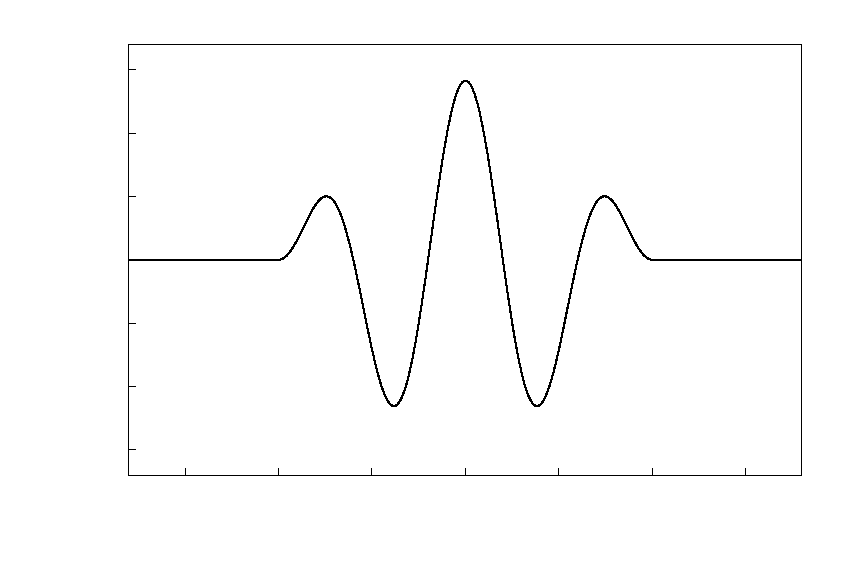
\includegraphics{psi}}%
    \gplfronttext
  \end{picture}%
\endgroup

\caption{$\psi(x)$ für $\alpha=\pi/4$ und $m=n+1=3$ sowie $\lambda=1$ in \emph{einheitenlosen} Größen.}
\label{fig:psi}
\end{figure}
\begin{figure}[htbp]
\centering
% GNUPLOT: LaTeX picture with Postscript
\begingroup
  \makeatletter
  \providecommand\color[2][]{%
    \GenericError{(gnuplot) \space\space\space\@spaces}{%
      Package color not loaded in conjunction with
      terminal option `colourtext'%
    }{See the gnuplot documentation for explanation.%
    }{Either use 'blacktext' in gnuplot or load the package
      color.sty in LaTeX.}%
    \renewcommand\color[2][]{}%
  }%
  \providecommand\includegraphics[2][]{%
    \GenericError{(gnuplot) \space\space\space\@spaces}{%
      Package graphicx or graphics not loaded%
    }{See the gnuplot documentation for explanation.%
    }{The gnuplot epslatex terminal needs graphicx.sty or graphics.sty.}%
    \renewcommand\includegraphics[2][]{}%
  }%
  \providecommand\rotatebox[2]{#2}%
  \@ifundefined{ifGPcolor}{%
    \newif\ifGPcolor
    \GPcolortrue
  }{}%
  \@ifundefined{ifGPblacktext}{%
    \newif\ifGPblacktext
    \GPblacktextfalse
  }{}%
  % define a \g@addto@macro without @ in the name:
  \let\gplgaddtomacro\g@addto@macro
  % define empty templates for all commands taking text:
  \gdef\gplbacktext{}%
  \gdef\gplfronttext{}%
  \makeatother
  \ifGPblacktext
    % no textcolor at all
    \def\colorrgb#1{}%
    \def\colorgray#1{}%
  \else
    % gray or color?
    \ifGPcolor
      \def\colorrgb#1{\color[rgb]{#1}}%
      \def\colorgray#1{\color[gray]{#1}}%
      \expandafter\def\csname LTw\endcsname{\color{white}}%
      \expandafter\def\csname LTb\endcsname{\color{black}}%
      \expandafter\def\csname LTa\endcsname{\color{black}}%
      \expandafter\def\csname LT0\endcsname{\color[rgb]{1,0,0}}%
      \expandafter\def\csname LT1\endcsname{\color[rgb]{0,1,0}}%
      \expandafter\def\csname LT2\endcsname{\color[rgb]{0,0,1}}%
      \expandafter\def\csname LT3\endcsname{\color[rgb]{1,0,1}}%
      \expandafter\def\csname LT4\endcsname{\color[rgb]{0,1,1}}%
      \expandafter\def\csname LT5\endcsname{\color[rgb]{1,1,0}}%
      \expandafter\def\csname LT6\endcsname{\color[rgb]{0,0,0}}%
      \expandafter\def\csname LT7\endcsname{\color[rgb]{1,0.3,0}}%
      \expandafter\def\csname LT8\endcsname{\color[rgb]{0.5,0.5,0.5}}%
    \else
      % gray
      \def\colorrgb#1{\color{black}}%
      \def\colorgray#1{\color[gray]{#1}}%
      \expandafter\def\csname LTw\endcsname{\color{white}}%
      \expandafter\def\csname LTb\endcsname{\color{black}}%
      \expandafter\def\csname LTa\endcsname{\color{black}}%
      \expandafter\def\csname LT0\endcsname{\color{black}}%
      \expandafter\def\csname LT1\endcsname{\color{black}}%
      \expandafter\def\csname LT2\endcsname{\color{black}}%
      \expandafter\def\csname LT3\endcsname{\color{black}}%
      \expandafter\def\csname LT4\endcsname{\color{black}}%
      \expandafter\def\csname LT5\endcsname{\color{black}}%
      \expandafter\def\csname LT6\endcsname{\color{black}}%
      \expandafter\def\csname LT7\endcsname{\color{black}}%
      \expandafter\def\csname LT8\endcsname{\color{black}}%
    \fi
  \fi
    \setlength{\unitlength}{0.0500bp}%
    \ifx\gptboxheight\undefined%
      \newlength{\gptboxheight}%
      \newlength{\gptboxwidth}%
      \newsavebox{\gptboxtext}%
    \fi%
    \setlength{\fboxrule}{0.5pt}%
    \setlength{\fboxsep}{1pt}%
\begin{picture}(7936.00,5102.00)%
    \gplgaddtomacro\gplbacktext{%
      \csname LTb\endcsname%
      \put(814,1048){\makebox(0,0)[r]{\strut{}$0$}}%
      \put(814,1909){\makebox(0,0)[r]{\strut{}$0.5$}}%
      \put(814,2770){\makebox(0,0)[r]{\strut{}$1$}}%
      \put(814,3632){\makebox(0,0)[r]{\strut{}$1.5$}}%
      \put(814,4493){\makebox(0,0)[r]{\strut{}$2$}}%
      \put(1495,484){\makebox(0,0){\strut{}$-1.5$}}%
      \put(2411,484){\makebox(0,0){\strut{}$-1$}}%
      \put(3327,484){\makebox(0,0){\strut{}$-0.5$}}%
      \put(4243,484){\makebox(0,0){\strut{}$0$}}%
      \put(5158,484){\makebox(0,0){\strut{}$0.5$}}%
      \put(6074,484){\makebox(0,0){\strut{}$1$}}%
      \put(6990,484){\makebox(0,0){\strut{}$1.5$}}%
    }%
    \gplgaddtomacro\gplfronttext{%
      \csname LTb\endcsname%
      \put(176,2770){\rotatebox{-270}{\makebox(0,0){\strut{}$|\psi(x)|^2$}}}%
      \put(4242,154){\makebox(0,0){\strut{}$x$}}%
    }%
    \gplgaddtomacro\gplbacktext{%
      \csname LTb\endcsname%
      \put(814,1048){\makebox(0,0)[r]{\strut{}$0$}}%
      \put(814,1909){\makebox(0,0)[r]{\strut{}$0.5$}}%
      \put(814,2770){\makebox(0,0)[r]{\strut{}$1$}}%
      \put(814,3632){\makebox(0,0)[r]{\strut{}$1.5$}}%
      \put(814,4493){\makebox(0,0)[r]{\strut{}$2$}}%
      \put(1495,484){\makebox(0,0){\strut{}$-1.5$}}%
      \put(2411,484){\makebox(0,0){\strut{}$-1$}}%
      \put(3327,484){\makebox(0,0){\strut{}$-0.5$}}%
      \put(4243,484){\makebox(0,0){\strut{}$0$}}%
      \put(5158,484){\makebox(0,0){\strut{}$0.5$}}%
      \put(6074,484){\makebox(0,0){\strut{}$1$}}%
      \put(6990,484){\makebox(0,0){\strut{}$1.5$}}%
    }%
    \gplgaddtomacro\gplfronttext{%
      \csname LTb\endcsname%
      \put(176,2770){\rotatebox{-270}{\makebox(0,0){\strut{}$|\psi(x)|^2$}}}%
      \put(4242,154){\makebox(0,0){\strut{}$x$}}%
    }%
    \gplbacktext
    \put(0,0){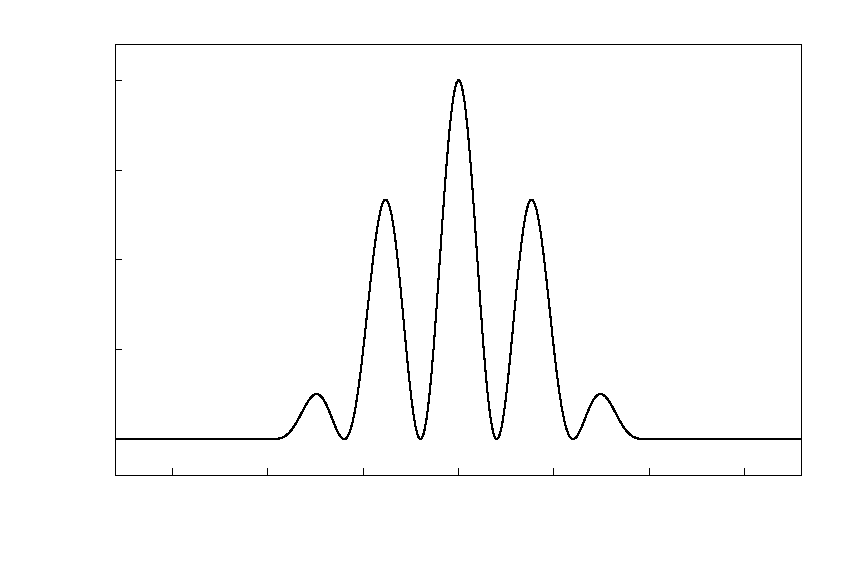
\includegraphics{psisquared}}%
    \gplfronttext
  \end{picture}%
\endgroup

\caption{$|\psi(x)|^2$ für $\alpha=\pi/4$ und $m=n+1=3$ sowie $\lambda=1$ in \emph{einheitenlosen} Größen.}
\label{fig:psisquared}
\end{figure}
\end{enumerate}